\chapter{Исследования}

\section{Предварительное описание}

Проведем сначала тестирование разработанной программы по векторному МКЭ на работоспособность. Образец расчетной области изображен на рисунке \ref{fig:exampleOfArea}. Это область $\Omega = [0.0, 3.0]_x \times [0.0, 3.0]_y \times [1.0, 2.0]_z$, она содержит 144 ребра, на всех границах будем задавать первые краевые условия. Ребра с глобальной нумерацией 48, 69, 70, 88, 51, 52, 91, 92, 55, 73, 74, 95 обозначены красным цветом, эти ребра мы будем учитывать при анализе на порядок сходмости и аппроксимации. 

\begin{figure}
	\centering
	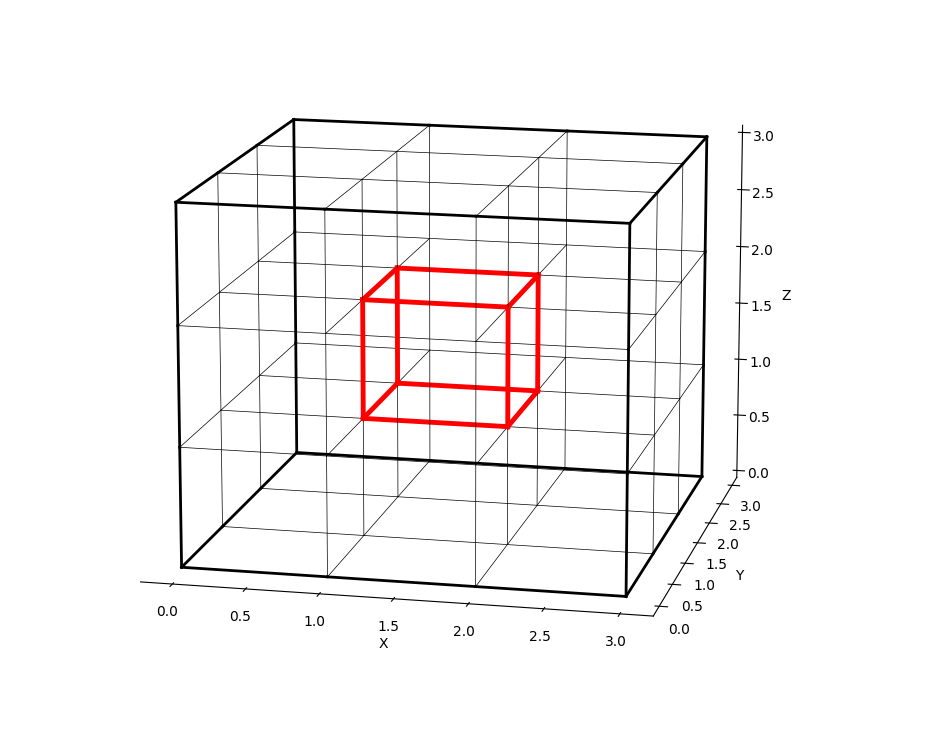
\includegraphics[width=1.0\linewidth]{images/3D_grid_example.png}
	\caption{Расчетная область}
	\label{fig:exampleOfArea}
\end{figure}

\section{Тестирование на порядок аппроксимации}

Тестирование будем проводить на дифференциальном уравнении (\ref{eq_2_1}) :

\begin{equation} \label{eq_2_1}
	\text{rot} \left(\frac{1}{\mu} \text{rot} \overrightarrow{\textbf{A}}\right) + \gamma \overrightarrow{\textbf{A}} = \overrightarrow{\textbf{F}}
\end{equation}

\begin{table}
	\caption{Тестирование при $\overrightarrow{\textbf{A}} = (1.0, 1.0, 1.0)^{\text{T}}$, $\overrightarrow{\textbf{F}} = (1.0, 1.0, 1.0)^{\text{T}}$, $\mu = 1$, $\gamma = 1$}
	\centering
	\small
	\begin{tabularx}{1.0\textwidth}{| >{\raggedright\arraybackslash}X | >{\raggedright\arraybackslash}X | >{\raggedright\arraybackslash}X |>{\raggedright\arraybackslash}X |}
		\hline
		\centering{Ребро} & \centering{Значение} & \centering{Абсолютная погрешность} & \centering{Относительная погрешность} \tabularnewline \hline
		

		 \centering{($x; 1.0; 1.0$)} & \centering{1.00000000E+000}& \centering{0.00000000E+000} & \centering{0.00000000E+000} \tabularnewline \hline
	
		 \centering{($x; 2.0; 1.0$)} & \centering{1.00000000E+000}& \centering{0.00000000E+000} & \centering{0.00000000E+000} \tabularnewline \hline

		 \centering{($x; 1.0; 2.0$)} & \centering{1.00000000E+000}& \centering{0.00000000E+000} & \centering{0.00000000E+000} \tabularnewline \hline

		 \centering{($x; 2.0; 2.0$)} & \centering{1.00000000E+000}& \centering{0.00000000E+000} & \centering{0.00000000E+000} \tabularnewline \hline



		 \centering{($1.0; y; 1.0$)} & \centering{1.00000000E+000}& \centering{0.00000000E+000} & \centering{0.00000000E+000} \tabularnewline \hline

		\centering{($2.0; y; 1.0$)} & \centering{1.00000000E+000}& \centering{0.00000000E+000} & \centering{0.00000000E+000} \tabularnewline \hline

		\centering{($1.0; y; 2.0$)} & \centering{1.00000000E+000}& \centering{0.00000000E+000} & \centering{0.00000000E+000} \tabularnewline \hline

		\centering{($2.0; y; 2.0$)} & \centering{1.00000000E+000}& \centering{0.00000000E+000} & \centering{0.00000000E+000} \tabularnewline \hline



		 \centering{($1.0; 1.0; z$)} & \centering{1.00000000E+000}& \centering{0.00000000E+000} & \centering{0.00000000E+000} \tabularnewline \hline

		 \centering{($2.0; 1.0; z$)} & \centering{1.00000000E+000}& \centering{0.00000000E+000} & \centering{0.00000000E+000} \tabularnewline \hline

		 \centering{($1.0; 2.0; z$)} & \centering{1.00000000E+000}& \centering{0.00000000E+000} & \centering{0.00000000E+000} \tabularnewline \hline

		 \centering{($2.0; 2.0; z$)} & \centering{1.00000000E+000}& \centering{0.00000000E+000} & \centering{0.00000000E+000} \tabularnewline \hline
		 

 	\end{tabularx}
	\label{tab:test1}
\end{table}

\begin{table}
	\caption{Тестирование при $\overrightarrow{\textbf{A}} = (y, z, x)^{\text{T}}$, $\overrightarrow{\textbf{F}} = (y, z, x)^{\text{T}}$, $\mu = 1$, $\gamma = 1$}
	\centering
	\small
	\begin{tabularx}{1.0\textwidth}{| >{\raggedright\arraybackslash}X | >{\raggedright\arraybackslash}X | >{\raggedright\arraybackslash}X |>{\raggedright\arraybackslash}X |}
		\hline
		\centering{Ребро} & \centering{Значение} & \centering{Абсолютная погрешность} & \centering{Относительная погрешность} \tabularnewline \hline
		
		 \centering{($x; 1.0; 1.0$)} & \centering{1.00000000E+000}& \centering{0.00000000E+000} & \centering{0.00000000E+000} \tabularnewline \hline

		\centering{($x; 2.0; 1.0$)} & \centering{2.00000000E+000}& \centering{0.00000000E+000} & \centering{0.00000000E+000} \tabularnewline \hline
	
		\centering{($x; 1.0; 2.0$)} & \centering{1.00000000E+000}& \centering{0.00000000E+000} & \centering{0.00000000E+000} \tabularnewline \hline
	
		\centering{($x; 2.0; 2.0$)} & \centering{2.00000000E+000}& \centering{0.00000000E+000} & \centering{0.00000000E+000} \tabularnewline \hline
	
	
	
		\centering{($1.0; y; 1.0$)} & \centering{1.00000000E+000}& \centering{0.00000000E+000} & \centering{0.00000000E+000} \tabularnewline \hline
	
		\centering{($2.0; y; 1.0$)} & \centering{1.00000000E+000}& \centering{0.00000000E+000} & \centering{0.00000000E+000} \tabularnewline \hline
	
		\centering{($1.0; y; 2.0$)} & \centering{2.00000000E+000}& \centering{0.00000000E+000} & \centering{0.00000000E+000} \tabularnewline \hline
	
		\centering{($2.0; y; 2.0$)} & \centering{2.00000000E+000}& \centering{0.00000000E+000} & \centering{0.00000000E+000} \tabularnewline \hline
	
	
	
		\centering{($1.0; 1.0; z$)} & \centering{1.00000000E+000}& \centering{0.00000000E+000} & \centering{0.00000000E+000} \tabularnewline \hline
	
		\centering{($2.0; 1.0; z$)} & \centering{2.00000000E+000}& \centering{0.00000000E+000} & \centering{0.00000000E+000} \tabularnewline \hline
	
		\centering{($1.0; 2.0; z$)} & \centering{1.00000000E+000}& \centering{0.00000000E+000} & \centering{0.00000000E+000} \tabularnewline \hline
	
		\centering{($2.0; 2.0; z$)} & \centering{2.00000000E+000}& \centering{0.00000000E+000} & \centering{0.00000000E+000} \tabularnewline \hline


	\end{tabularx}
	\label{tab:test2}
\end{table}

\begin{table}
\caption{Тестирование при $\overrightarrow{\textbf{A}} = (1 + y + x; 1 + x + z; 1 + x + y)^{\text{T}}$, $\overrightarrow{\textbf{F}} = (1 + y + x; 1 + x + z; 1 + x + y)^{\text{T}}$, $\mu = 1$, $\gamma = 1$}
\centering
\small
\begin{tabularx}{1.0\textwidth}{| >{\raggedright\arraybackslash}X | >{\raggedright\arraybackslash}X | >{\raggedright\arraybackslash}X |>{\raggedright\arraybackslash}X |}
	\hline
		\centering{Ребро} & \centering{Значение} & \centering{Абсолютная погрешность} & \centering{Относительная погрешность} \tabularnewline \hline
	
	
		 \centering{($x; 1.0; 1.0$)} & \centering{3.00000000E+000}& \centering{0.00000000E+000} & \centering{0.00000000E+000} \tabularnewline \hline

		\centering{($x; 2.0; 1.0$)} & \centering{4.00000000E+000}& \centering{0.00000000E+000} & \centering{0.00000000E+000} \tabularnewline \hline

		\centering{($x; 1.0; 2.0$)} & \centering{4.00000000E+000}& \centering{0.00000000E+000} & \centering{0.00000000E+000} \tabularnewline \hline

		\centering{($x; 2.0; 2.0$)} & \centering{5.00000000E+000}& \centering{0.00000000E+000} & \centering{0.00000000E+000} \tabularnewline \hline



		\centering{($1.0; y; 1.0$)} & \centering{3.00000000E+000}& \centering{0.00000000E+000} & \centering{0.00000000E+000} \tabularnewline \hline

		\centering{($2.0; y; 1.0$)} & \centering{4.00000000E+000}& \centering{0.00000000E+000} & \centering{0.00000000E+000} \tabularnewline \hline

		\centering{($1.0; y; 2.0$)} & \centering{4.00000000E+000}& \centering{0.00000000E+000} & \centering{0.00000000E+000} \tabularnewline \hline

		\centering{($2.0; y; 2.0$)} & \centering{5.00000000E+000}& \centering{0.00000000E+000} & \centering{0.00000000E+000} \tabularnewline \hline



		\centering{($1.0; 1.0; z$)} & \centering{3.00000000E+000}& \centering{0.00000000E+000} & \centering{0.00000000E+000} \tabularnewline \hline

		\centering{($2.0; 1.0; z$)} & \centering{4.00000000E+000}& \centering{0.00000000E+000} & \centering{0.00000000E+000} \tabularnewline \hline

		\centering{($1.0; 2.0; z$)} & \centering{4.00000000E+000}& \centering{0.00000000E+000} & \centering{0.00000000E+000} \tabularnewline \hline

		\centering{($2.0; 2.0; z$)} & \centering{5.00000000E+000}& \centering{0.00000000E+000} & \centering{0.00000000E+000} \tabularnewline \hline
	
\end{tabularx}
\label{tab:test3}
\end{table}

\begin{table}
\caption{Тестирование при $\overrightarrow{\textbf{A}} = (y - z; x - z; x - y)^{\text{T}}$, $\overrightarrow{\textbf{F}} = (y - x; x - z; x - y)^{\text{T}}$, $\mu = 1$, $\gamma = 1$}
\centering
\small
\begin{tabularx}{1.0\textwidth}{| >{\raggedright\arraybackslash}X | >{\raggedright\arraybackslash}X | >{\raggedright\arraybackslash}X |>{\raggedright\arraybackslash}X |}
	\hline
		\centering{Ребро} & \centering{Значение} & \centering{Абсолютная погрешность} & \centering{Относительная погрешность} \tabularnewline \hline


		\centering{($x; 1.0; 1.0$)} & \centering{2.35132600E-016}& \centering{2.35132600E-016} & \centering{0.00000000E+000} \tabularnewline \hline

		\centering{($x; 2.0; 1.0$)} & \centering{1.00000000E+000}& \centering{0.00000000E+000} & \centering{0.00000000E+000} \tabularnewline \hline

		\centering{($x; 1.0; 2.0$)} & \centering{-1.00000000E+000}& \centering{0.00000000E+000} & \centering{0.00000000E+000} \tabularnewline \hline

		\centering{($x; 2.0; 2.0$)} & \centering{-5.55111512E-016}& \centering{-5.55111512E-016} & \centering{0.00000000E+000} \tabularnewline \hline



		\centering{($1.0; y; 1.0$)} & \centering{-3.97378607E-016}& \centering{-3.97378607E-016} & \centering{0.00000000E+000} \tabularnewline \hline

		\centering{($2.0; y; 1.0$)} & \centering{1.00000000E+000}& \centering{0.00000000E+000} & \centering{0.00000000E+000} \tabularnewline \hline

		\centering{($1.0; y; 2.0$)} & \centering{-1.00000000E+000}& \centering{0.00000000E+000} & \centering{0.00000000E+000} \tabularnewline \hline

		\centering{($2.0; y; 2.0$)} & \centering{-1.94289029E-016}& \centering{-1.94289029E-016} & \centering{0.00000000E+000} \tabularnewline \hline



		\centering{($1.0; 1.0; z$)} & \centering{-2.74847895E-016}& \centering{-2.74847895E-016} & \centering{0.00000000E+000} \tabularnewline \hline

		\centering{($2.0; 1.0; z$)} & \centering{1.00000000E+000}& \centering{0.00000000E+000} & \centering{0.00000000E+000} \tabularnewline \hline

		\centering{($1.0; 2.0; z$)} & \centering{-1.00000000E+000}& \centering{0.00000000E+000} & \centering{0.00000000E+000} \tabularnewline \hline

		\centering{($2.0; 2.0; z$)} & \centering{4.27842044E-016}& \centering{4.27842044E-016} & \centering{0.00000000E+000} \tabularnewline \hline

	
\end{tabularx}
\label{tab:test4}
\end{table}

\begin{table}
\caption{Тестирование при $\overrightarrow{\textbf{A}} = (y \cdot z; x \cdot z; x \cdot y)^{\text{T}}$, $\overrightarrow{\textbf{F}} = (y \cdot z; x \cdot z; x \cdot y)^{\text{T}}$, $\mu = 1$, $\gamma = 1$}
\centering
\small
\begin{tabularx}{1.0\textwidth}{| >{\raggedright\arraybackslash}X | >{\raggedright\arraybackslash}X | >{\raggedright\arraybackslash}X |>{\raggedright\arraybackslash}X |}
	\hline
	\centering{Ребро} & \centering{Значение} & \centering{Абсолютная погрешность} & \centering{Относительная погрешность} \tabularnewline \hline
	
	
	\centering{($x; 1.0; 1.0$)} & \centering{1.00000000E+000}& \centering{0.00000000E+000} & \centering{0.00000000E+000} \tabularnewline \hline
	
	\centering{($x; 2.0; 1.0$)} & \centering{2.00000000E+000}& \centering{0.00000000E+000} & \centering{0.00000000E+000} \tabularnewline \hline
	
	\centering{($x; 1.0; 2.0$)} & \centering{2.00000000E+000}& \centering{0.00000000E+000} & \centering{0.00000000E+000} \tabularnewline \hline
	
	\centering{($x; 2.0; 2.0$)} & \centering{4.00000000E+000}& \centering{0.00000000E+000} & \centering{0.00000000E+000} \tabularnewline \hline
	
	
	
	\centering{($1.0; y; 1.0$)} & \centering{1.00000000E+000}& \centering{0.00000000E+000} & \centering{0.00000000E+000} \tabularnewline \hline
	
	\centering{($2.0; y; 1.0$)} & \centering{2.00000000E+000}& \centering{0.00000000E+000} & \centering{0.00000000E+000} \tabularnewline \hline
	
	\centering{($1.0; y; 2.0$)} & \centering{2.00000000E+000}& \centering{0.00000000E+000} & \centering{0.00000000E+000} \tabularnewline \hline
	
	\centering{($2.0; y; 2.0$)} & \centering{4.00000000E+000}& \centering{0.00000000E+000} & \centering{0.00000000E+000} \tabularnewline \hline
	
	
	
	\centering{($1.0; 1.0; z$)} & \centering{1.00000000E+000}& \centering{0.00000000E+000} & \centering{0.00000000E+000} \tabularnewline \hline
	
	\centering{($2.0; 1.0; z$)} & \centering{2.00000000E+000}& \centering{0.00000000E+000} & \centering{0.00000000E+000} \tabularnewline \hline
	
	\centering{($1.0; 2.0; z$)} & \centering{2.00000000E+000}& \centering{0.00000000E+000} & \centering{0.00000000E+000} \tabularnewline \hline
	
	\centering{($2.0; 2.0; z$)} & \centering{4.00000000E+000}& \centering{0.00000000E+000} & \centering{0.00000000E+000} \tabularnewline \hline
	
\end{tabularx}
\label{tab:test5}
\end{table}

\begin{table}
\caption{Тестирование при $\overrightarrow{\textbf{A}} = (y^2; z^2; x^2)^{\text{T}}$, $\overrightarrow{\textbf{F}} = (y^2 - 2; z^2 - 2; x^2 - 2)^{\text{T}}$, $\mu = 1$, $\gamma = 1$}
\centering
\small
\begin{tabularx}{1.0\textwidth}{| >{\raggedright\arraybackslash}X | >{\raggedright\arraybackslash}X | >{\raggedright\arraybackslash}X |>{\raggedright\arraybackslash}X |}
	\hline
	\centering{Ребро} & \centering{Значение} & \centering{Абсолютная погрешность} & \centering{Относительная погрешность} \tabularnewline \hline


	\centering{($x; 1.0; 1.0$)} & \centering{1.00000000E+000}& \centering{0.00000000E+000} & \centering{0.00000000E+000} \tabularnewline \hline

	\centering{($x; 2.0; 1.0$)} & \centering{4.00000000E+000}& \centering{0.00000000E+000} & \centering{0.00000000E+000} \tabularnewline \hline

	\centering{($x; 1.0; 2.0$)} & \centering{1.00000000E+000}& \centering{0.00000000E+000} & \centering{0.00000000E+000} \tabularnewline \hline

	\centering{($x; 2.0; 2.0$)} & \centering{4.00000000E+000}& \centering{0.00000000E+000} & \centering{0.00000000E+000} \tabularnewline \hline



	\centering{($1.0; y; 1.0$)} & \centering{1.00000000E+000}& \centering{0.00000000E+000} & \centering{0.00000000E+000} \tabularnewline \hline

	\centering{($2.0; y; 1.0$)} & \centering{1.00000000E+000}& \centering{0.00000000E+000} & \centering{0.00000000E+000} \tabularnewline \hline

	\centering{($1.0; y; 2.0$)} & \centering{4.00000000E+000}& \centering{0.00000000E+000} & \centering{0.00000000E+000} \tabularnewline \hline

	\centering{($2.0; y; 2.0$)} & \centering{4.00000000E+000}& \centering{0.00000000E+000} & \centering{0.00000000E+000} \tabularnewline \hline



	\centering{($1.0; 1.0; z$)} & \centering{1.00000000E+000}& \centering{0.00000000E+000} & \centering{0.00000000E+000} \tabularnewline \hline

	\centering{($2.0; 1.0; z$)} & \centering{4.00000000E+000}& \centering{0.00000000E+000} & \centering{0.00000000E+000} \tabularnewline \hline

	\centering{($1.0; 2.0; z$)} & \centering{1.00000000E+000}& \centering{0.00000000E+000} & \centering{0.00000000E+000} \tabularnewline \hline

	\centering{($2.0; 2.0; z$)} & \centering{4.00000000E+000}& \centering{0.00000000E+000} & \centering{0.00000000E+000} \tabularnewline \hline
\end{tabularx}
\label{tab:test6}
\end{table}

\begin{table}
\caption{Тестирование при $\overrightarrow{\textbf{A}} = (y^2 + z^2; x^2 + z^2; x^2 + y^2)^{\text{T}}$, $\overrightarrow{\textbf{F}} = (y^2 + z^2 - 4; x^2 + z^2 - 4; x^2 + y^2 - 4)^{\text{T}}$, $\mu = 1$, $\gamma = 1$}
\centering
\small
\begin{tabularx}{1.0\textwidth}{| >{\raggedright\arraybackslash}X | >{\raggedright\arraybackslash}X | >{\raggedright\arraybackslash}X |>{\raggedright\arraybackslash}X |}
	\hline
	\centering{Ребро} & \centering{Значение} & \centering{Абсолютная погрешность} & \centering{Относительная погрешность} \tabularnewline \hline


\centering{($x; 1.0; 1.0$)} & \centering{2.00000000E+000}& \centering{0.00000000E+000} & \centering{0.00000000E+000} \tabularnewline \hline

\centering{($x; 2.0; 1.0$)} & \centering{5.00000000E+000}& \centering{0.00000000E+000} & \centering{0.00000000E+000} \tabularnewline \hline

\centering{($x; 1.0; 2.0$)} & \centering{5.00000000E+000}& \centering{0.00000000E+000} & \centering{0.00000000E+000} \tabularnewline \hline

\centering{($x; 2.0; 2.0$)} & \centering{8.00000000E+000}& \centering{0.00000000E+000} & \centering{0.00000000E+000} \tabularnewline \hline



\centering{($1.0; y; 1.0$)} & \centering{2.00000000E+000}& \centering{0.00000000E+000} & \centering{0.00000000E+000} \tabularnewline \hline

\centering{($2.0; y; 1.0$)} & \centering{5.00000000E+000}& \centering{0.00000000E+000} & \centering{0.00000000E+000} \tabularnewline \hline

\centering{($1.0; y; 2.0$)} & \centering{5.00000000E+000}& \centering{0.00000000E+000} & \centering{0.00000000E+000} \tabularnewline \hline

\centering{($2.0; y; 2.0$)} & \centering{8.00000000E+000}& \centering{0.00000000E+000} & \centering{0.00000000E+000} \tabularnewline \hline



\centering{($1.0; 1.0; z$)} & \centering{2.00000000E+000}& \centering{0.00000000E+000} & \centering{0.00000000E+000} \tabularnewline \hline

\centering{($2.0; 1.0; z$)} & \centering{5.00000000E+000}& \centering{0.00000000E+000} & \centering{0.00000000E+000} \tabularnewline \hline

\centering{($1.0; 2.0; z$)} & \centering{5.00000000E+000}& \centering{0.00000000E+000} & \centering{0.00000000E+000} \tabularnewline \hline

\centering{($2.0; 2.0; z$)} & \centering{8.00000000E+000}& \centering{0.00000000E+000} & \centering{0.00000000E+000} \tabularnewline \hline
	
\end{tabularx}
\label{tab:test7}
\end{table}

\begin{table}
\caption{Тестирование при $\overrightarrow{\textbf{A}} = (y^3; 0; 0)^{\text{T}}$, $\overrightarrow{\textbf{F}} = (y^3 - 6y; 0; 0)^{\text{T}}$, $\mu = 1$, $\gamma = 1$}
\centering
\small
\begin{tabularx}{1.0\textwidth}{| >{\raggedright\arraybackslash}X | >{\raggedright\arraybackslash}X | >{\raggedright\arraybackslash}X |>{\raggedright\arraybackslash}X |}
	\hline
	\centering{Ребро} & \centering{Значение} & \centering{Абсолютная погрешность} & \centering{Относительная погрешность} \tabularnewline \hline


\centering{($x; 1.0; 1.0$)} & \centering{1.00000000E+000}& \centering{0.00000000E+000} & \centering{0.00000000E+000} \tabularnewline \hline

\centering{($x; 2.0; 1.0$)} & \centering{8.00000000E+000}& \centering{0.00000000E+000} & \centering{0.00000000E+000} \tabularnewline \hline

\centering{($x; 1.0; 2.0$)} & \centering{1.00000000E+000}& \centering{0.00000000E+000} & \centering{0.00000000E+000} \tabularnewline \hline

\centering{($x; 2.0; 2.0$)} & \centering{8.00000000E+000}& \centering{0.00000000E+000} & \centering{0.00000000E+000} \tabularnewline \hline



\centering{($1.0; y; 1.0$)} & \centering{0.00000000E+000}& \centering{0.00000000E+000} & \centering{0.00000000E+000} \tabularnewline \hline

\centering{($2.0; y; 1.0$)} & \centering{0.00000000E+000}& \centering{0.00000000E+000} & \centering{0.00000000E+000} \tabularnewline \hline

\centering{($1.0; y; 2.0$)} & \centering{0.00000000E+000}& \centering{0.00000000E+000} & \centering{0.00000000E+000} \tabularnewline \hline

\centering{($2.0; y; 2.0$)} & \centering{0.00000000E+000}& \centering{0.00000000E+000} & \centering{0.00000000E+000} \tabularnewline \hline



\centering{($1.0; 1.0; z$)} & \centering{0.00000000E+000}& \centering{0.00000000E+000} & \centering{0.00000000E+000} \tabularnewline \hline

\centering{($2.0; 1.0; z$)} & \centering{0.00000000E+000}& \centering{0.00000000E+000} & \centering{0.00000000E+000} \tabularnewline \hline

\centering{($1.0; 2.0; z$)} & \centering{0.00000000E+000}& \centering{0.00000000E+000} & \centering{0.00000000E+000} \tabularnewline \hline

\centering{($2.0; 2.0; z$)} & \centering{0.00000000E+000}& \centering{0.00000000E+000} & \centering{0.00000000E+000} \tabularnewline \hline
	
\end{tabularx}
\label{tab:test8}
\end{table}

\begin{table}
\caption{Тестирование при $\overrightarrow{\textbf{A}} = (y^2 \cdot z^2; x^2 \cdot z^2; x^2 \cdot y^2)^{\text{T}}$, $\overrightarrow{\textbf{F}} = (y^2 \cdot z^2 - 2(y^2 + z^2); x^2 \cdot z^2 - 2(x^2 + z^2); x^2 \cdot y^2 - 2(x^2 + y^2))^{\text{T}}$, $\mu = 1$, $\gamma = 1$}
\centering
\small
\begin{tabularx}{1.0\textwidth}{| >{\raggedright\arraybackslash}X | >{\raggedright\arraybackslash}X | >{\raggedright\arraybackslash}X |>{\raggedright\arraybackslash}X |}
	\hline
	\centering{Ребро} & \centering{Значение} & \centering{Абсолютная погрешность} & \centering{Относительная погрешность} \tabularnewline \hline


\centering{($x; 1.0; 1.0$)} & \centering{1.00000000E+000}& \centering{0.00000000E+000} & \centering{0.00000000E+000} \tabularnewline \hline

\centering{($x; 2.0; 1.0$)} & \centering{4.00000000E+000}& \centering{0.00000000E+000} & \centering{0.00000000E+000} \tabularnewline \hline

\centering{($x; 1.0; 2.0$)} & \centering{4.00000000E+000}& \centering{0.00000000E+000} & \centering{0.00000000E+000} \tabularnewline \hline

\centering{($x; 2.0; 2.0$)} & \centering{1.60000000E+001}& \centering{0.00000000E+000} & \centering{0.00000000E+000} \tabularnewline \hline



\centering{($1.0; y; 1.0$)} & \centering{1.00000000E+000}& \centering{0.00000000E+000} & \centering{0.00000000E+000} \tabularnewline \hline

\centering{($2.0; y; 1.0$)} & \centering{4.00000000E+000}& \centering{0.00000000E+000} & \centering{0.00000000E+000} \tabularnewline \hline

\centering{($1.0; y; 2.0$)} & \centering{4.00000000E+000}& \centering{0.00000000E+000} & \centering{0.00000000E+000} \tabularnewline \hline

\centering{($2.0; y; 2.0$)} & \centering{1.60000000E+001}& \centering{0.00000000E+000} & \centering{0.00000000E+000} \tabularnewline \hline



\centering{($1.0; 1.0; z$)} & \centering{1.00000000E+000}& \centering{0.00000000E+000} & \centering{0.00000000E+000} \tabularnewline \hline

\centering{($2.0; 1.0; z$)} & \centering{4.00000000E+000}& \centering{0.00000000E+000} & \centering{0.00000000E+000} \tabularnewline \hline

\centering{($1.0; 2.0; z$)} & \centering{4.00000000E+000}& \centering{0.00000000E+000} & \centering{0.00000000E+000} \tabularnewline \hline

\centering{($2.0; 2.0; z$)} & \centering{1.60000000E+001}& \centering{0.00000000E+000} & \centering{0.00000000E+000} \tabularnewline \hline
	
\end{tabularx}
\label{tab:test9}
\end{table}

Далее проведем тесты нестационарной задачи (\ref{eq_2_2}):


\begin{equation} \label{eq_2_2}
	\text{rot} \left(\frac{1}{\mu} \text{rot} \overrightarrow{\textbf{A}}\right) + \gamma \overrightarrow{\textbf{A}} + \sigma \frac{\partial \overrightarrow{\textbf{A}}}{\partial t} = \overrightarrow{\textbf{F}}
\end{equation}

\begin{table}
	\caption{Тестирование при $\overrightarrow{\textbf{A}} = (y; z; x)^{\text{T}}$, $\overrightarrow{\textbf{F}} = (y; z; x)^{\text{T}}$, $\mu = 1$, $\gamma = 1$,  $\sigma = 1$}
	\centering
	\small
	\begin{tabularx}{1.0\textwidth}{| >{\raggedright\arraybackslash}X | >{\raggedright\arraybackslash}X | >{\raggedright\arraybackslash}X |>{\raggedright\arraybackslash}X |}
		\hline
		\centering{Ребро \newline $(x_c, y_c, z_c, t)$} & \centering{Значение} & \centering{Абсолютная погрешность} & \centering{Относительная погрешность} \tabularnewline \hline
		
		
		\centering{($x; 1.0; 1.0; 0.0$)} & \centering{1.00000000E+000}& \centering{0.00000000E+000} & \centering{0.00000000E+000} \tabularnewline 
		
		\centering{($x; 2.0; 2.0; 0.0$)} & \centering{1.60000000E+001}& \centering{0.00000000E+000} & \centering{0.00000000E+000} \tabularnewline 
		
		
		
		\centering{($1.0; y; 1.0; 0.0$)} & \centering{1.00000000E+000}& \centering{0.00000000E+000} & \centering{0.00000000E+000} \tabularnewline 
		
		\centering{($2.0; y; 2.0; 0.0$)} & \centering{1.60000000E+001}& \centering{0.00000000E+000} & \centering{0.00000000E+000} \tabularnewline 
		
		
		
		\centering{($1.0; 1.0; z; 0.0$)} & \centering{1.00000000E+000}& \centering{0.00000000E+000} & \centering{0.00000000E+000} \tabularnewline 

		\centering{($2.0; 2.0; z; 0.0$)} & \centering{1.60000000E+001}& \centering{0.00000000E+000} & \centering{0.00000000E+000} \tabularnewline \hline
		
		
		\centering{($x; 1.0; 1.0; 1.0$)} & \centering{1.00000000E+000}& \centering{0.00000000E+000} & \centering{0.00000000E+000} \tabularnewline 
		
		\centering{($x; 2.0; 2.0; 1.0$)} & \centering{1.60000000E+001}& \centering{0.00000000E+000} & \centering{0.00000000E+000} \tabularnewline 
		
		
		
		\centering{($1.0; y; 1.0; 1.0$)} & \centering{1.00000000E+000}& \centering{0.00000000E+000} & \centering{0.00000000E+000} \tabularnewline 
		
		\centering{($2.0; y; 2.0; 0.0$)} & \centering{1.60000000E+001}& \centering{0.00000000E+000} & \centering{0.00000000E+000} \tabularnewline 
		
		
		
		\centering{($1.0; 1.0; z; 1.0$)} & \centering{1.00000000E+000}& \centering{0.00000000E+000} & \centering{0.00000000E+000} \tabularnewline 
		
		\centering{($2.0; 2.0; z; 1.0$)} & \centering{1.60000000E+001}& \centering{0.00000000E+000} & \centering{0.00000000E+000} \tabularnewline \hline
		
		
		
		\centering{($x; 1.0; 1.0; 2.0$)} & \centering{1.00000000E+000}& \centering{0.00000000E+000} & \centering{0.00000000E+000} \tabularnewline 
		
		\centering{($x; 2.0; 2.0; 2.0$)} & \centering{1.60000000E+001}& \centering{0.00000000E+000} & \centering{0.00000000E+000} \tabularnewline 
		
		
		
		\centering{($1.0; y; 1.0; 2.0$)} & \centering{1.00000000E+000}& \centering{0.00000000E+000} & \centering{0.00000000E+000} \tabularnewline 
		
		\centering{($2.0; y; 2.0; 2.0$)} & \centering{1.60000000E+001}& \centering{0.00000000E+000} & \centering{0.00000000E+000} \tabularnewline 
		
		
		
		\centering{($1.0; 1.0; z; 2.0$)} & \centering{1.00000000E+000}& \centering{0.00000000E+000} & \centering{0.00000000E+000} \tabularnewline 
		
		\centering{($2.0; 2.0; z; 2.0$)} & \centering{1.60000000E+001}& \centering{0.00000000E+000} & \centering{0.00000000E+000} \tabularnewline \hline
		
		
		
		\centering{($x; 1.0; 1.0; 3.0$)} & \centering{1.00000000E+000}& \centering{0.00000000E+000} & \centering{0.00000000E+000} \tabularnewline 
		
		\centering{($x; 2.0; 2.0; 3.0$)} & \centering{1.60000000E+001}& \centering{0.00000000E+000} & \centering{0.00000000E+000} \tabularnewline 
		
		
		
		\centering{($1.0; y; 1.0; 3.0$)} & \centering{1.00000000E+000}& \centering{0.00000000E+000} & \centering{0.00000000E+000} \tabularnewline 
		
		\centering{($2.0; y; 2.0; 3.0$)} & \centering{1.60000000E+001}& \centering{0.00000000E+000} & \centering{0.00000000E+000} \tabularnewline 
		
		
		
		\centering{($1.0; 1.0; z; 3.0$)} & \centering{1.00000000E+000}& \centering{0.00000000E+000} & \centering{0.00000000E+000} \tabularnewline 
		
		\centering{($2.0; 2.0; z; 3.0$)} & \centering{1.60000000E+001}& \centering{0.00000000E+000} & \centering{0.00000000E+000} \tabularnewline \hline
		
		\centering{($x; 1.0; 1.0; 4.0$)} & \centering{1.00000000E+000}& \centering{0.00000000E+000} & \centering{0.00000000E+000} \tabularnewline 
		
		\centering{($x; 2.0; 2.0; 4.0$)} & \centering{1.60000000E+001}& \centering{0.00000000E+000} & \centering{0.00000000E+000} \tabularnewline 
		
		
		
		\centering{($1.0; y; 1.0; 4.0$)} & \centering{1.00000000E+000}& \centering{0.00000000E+000} & \centering{0.00000000E+000} \tabularnewline 
		
		\centering{($2.0; y; 2.0; 4.0$)} & \centering{1.60000000E+001}& \centering{0.00000000E+000} & \centering{0.00000000E+000} \tabularnewline 
		
		
		
		\centering{($1.0; 1.0; z; 4.0$)} & \centering{1.00000000E+000}& \centering{0.00000000E+000} & \centering{0.00000000E+000} \tabularnewline 
		
		\centering{($2.0; 2.0; z; 4.0$)} & \centering{1.60000000E+001}& \centering{0.00000000E+000} & \centering{0.00000000E+000} \tabularnewline \hline
		
	\end{tabularx}
	\label{tab:test10}
\end{table}

Исходя из полученных данных, можно сказать, что программа верно находит численное решение эллиптической задачи.
